%!TEX root = ../main.tex

\chapter{Experimental Evaluation}
\label{ch:eval}

\section{Use case}
To simulate the system functionality a case for two persons from different organizations trying to issue and mint data, send it and making it available to one another.

\section{Experimental Setup and Data Set}
\subsection{Scenario}
Simulation of two organizations willing to share data with each other.
\subsubsection{Organization 1}
Represents an organization with important information gathered from external resources, expensive and difficult to obtain. Has the technology and infrastructure to generate data, but does not count with the know how neither infrastructure to process it or exploit it (similar to machine learning / big data scenarios).

\textbf{User 'Minter'}
"Organization 1" Creates a user "Minter" as a company representative in charge of submitting the data and creating a \ac{NFT} version of it inside the system. Then he can use the system to lend the data, enable a time frame visualization or transfer it.

\subsubsection{Organization 2}
Represents a technology company with skillful personal in data processing and domain area in the business of "Organization 1", but does not have the experience nor technology to gather it. Therefore it needs data from the aforementioned organization in order to create and expand their business.

\textbf{User 'Receiver'}
"Organization 2" Creates a user "Receiver"  as a company representative in charge of getting access to the \ac{NFT} minted data by "Organization 1" via user "Minter" which will be used as the data source to perform machine learning training operations. 

With the use of the NFT System framework these parties can cooperate and participate by trusting that the information is secure, has not been altered and can be easily verified by them and other parties.

\section{Experimental Results}
The complete simulation of the process is shown in this section.

\subsection{System registering and user enrollment}
The NFT system provides a friendly user interface to allow organizations to be registered into the Fabric network to use a specific channel. 
Prior to this process Fabric generated a \ac{CA} with which they can identify as trusted entities and fair participants of the network.

The first time an organization registers itself to join a private channel, an admin account is created. The admin account then is able to configure organization parameters and new users with restricted access or different mining/system-usage capabilities.
in the figure \ref{fig:SeqDiag_RegisterEnroll} can be visualized the process any organization will take to register itself as a valid participant with its corresponding representatives.

 \begin{figure}[!h]
        \centering
        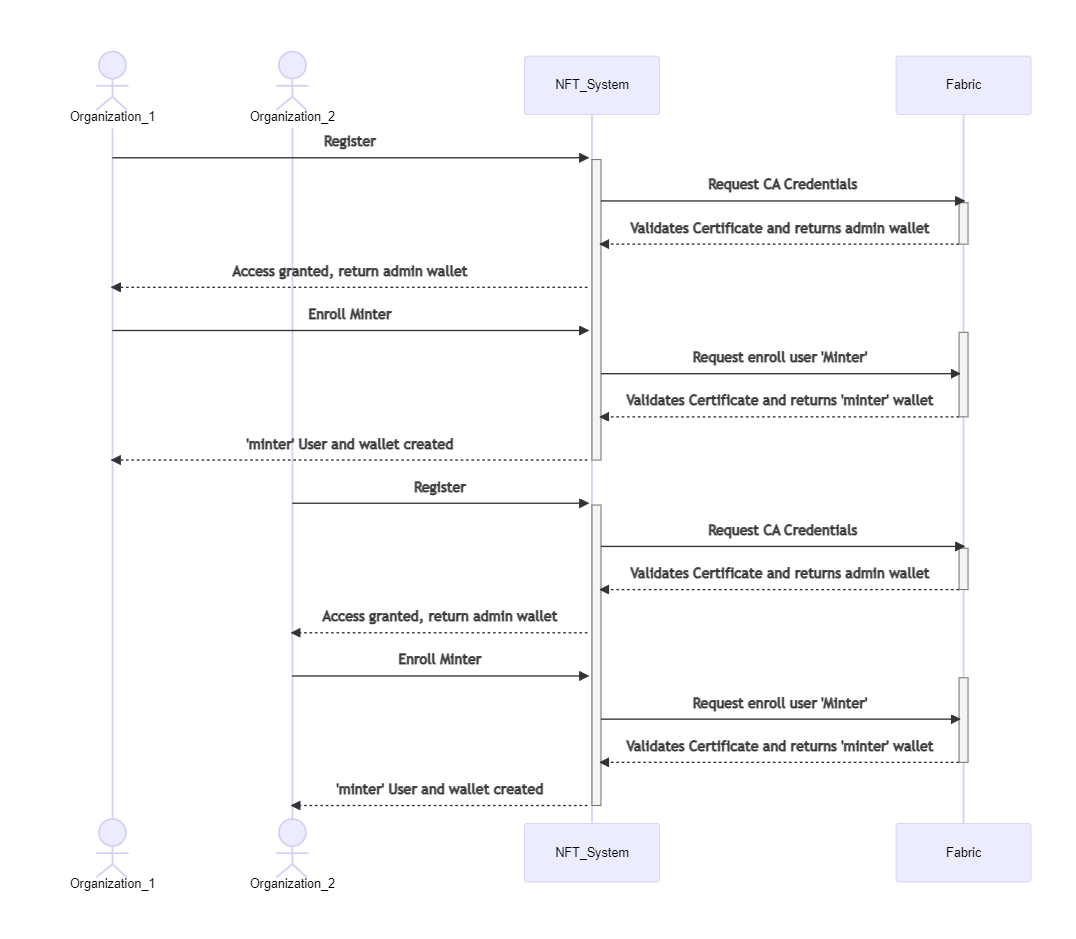
\includegraphics[width=15cm]{img/SequenceDiagram_RegisterEnroll.png}
        \caption{Sequence diagram of the Organization and user enrollment process in the system.}
        \label{fig:SeqDiag_RegisterEnroll}
    \end{figure}


 \begin{figure}[!h]
        \centering
        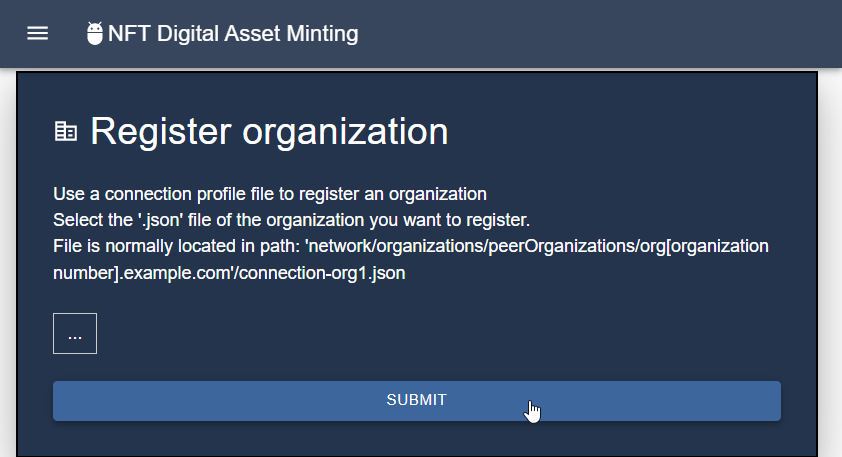
\includegraphics[width=7cm]{img/NFT_REGISTER.png}
        \caption{UI Register organization.}
        \label{fig:UI_Register}
    \end{figure}


 \begin{figure}[!h]
        \centering
        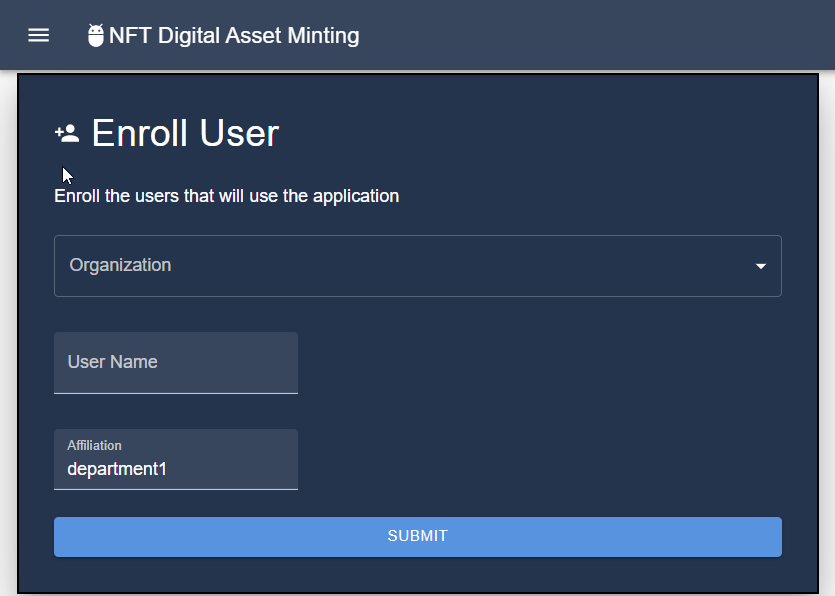
\includegraphics[width=7cm]{img/NFT_ENROLL.png}
        \caption{UI Enroll Users.}
        \label{fig:UI_Enroll}
    \end{figure}

\hfill \break

\subsection{NFT Minting and data reading access}
Once the organizations and users have been properly enrolled it the following steps must occur:
\begin{enumerate}
    \item Minter access to the platform and selects the "Mint 
    \ac{NFT} option.
    \item Minter selects a file and completes the form metadata.
    \item Minter clocks on "submit" button to create the token.
    \item The System talks verifies that the file does not exist yet by:
    \begin{itemize}
        \item Asking to add the data file to the \ac{IPFS} network
        \item Asking to Fabric if there is any token with the corresponding \ac{CID}
    \end{itemize}
    For any of those cases to be true, the token will not be generated and an error will be returned.
    \item Once everything is approved the token is stored in the \ac{DLT} with the corresponding file \ac{CID} generated.
    \item 'Minter' can now send the \ac{CID} or additional token information to 'Receiver'. Then receiver can pull such information from the infrastructure. Because of its unicity purposes 'Receiver' will not be able to counterfeit or take ownership of the data unless explicitly stipulated and agreed by both parties.
\end{enumerate}

 \begin{figure}[!h]
        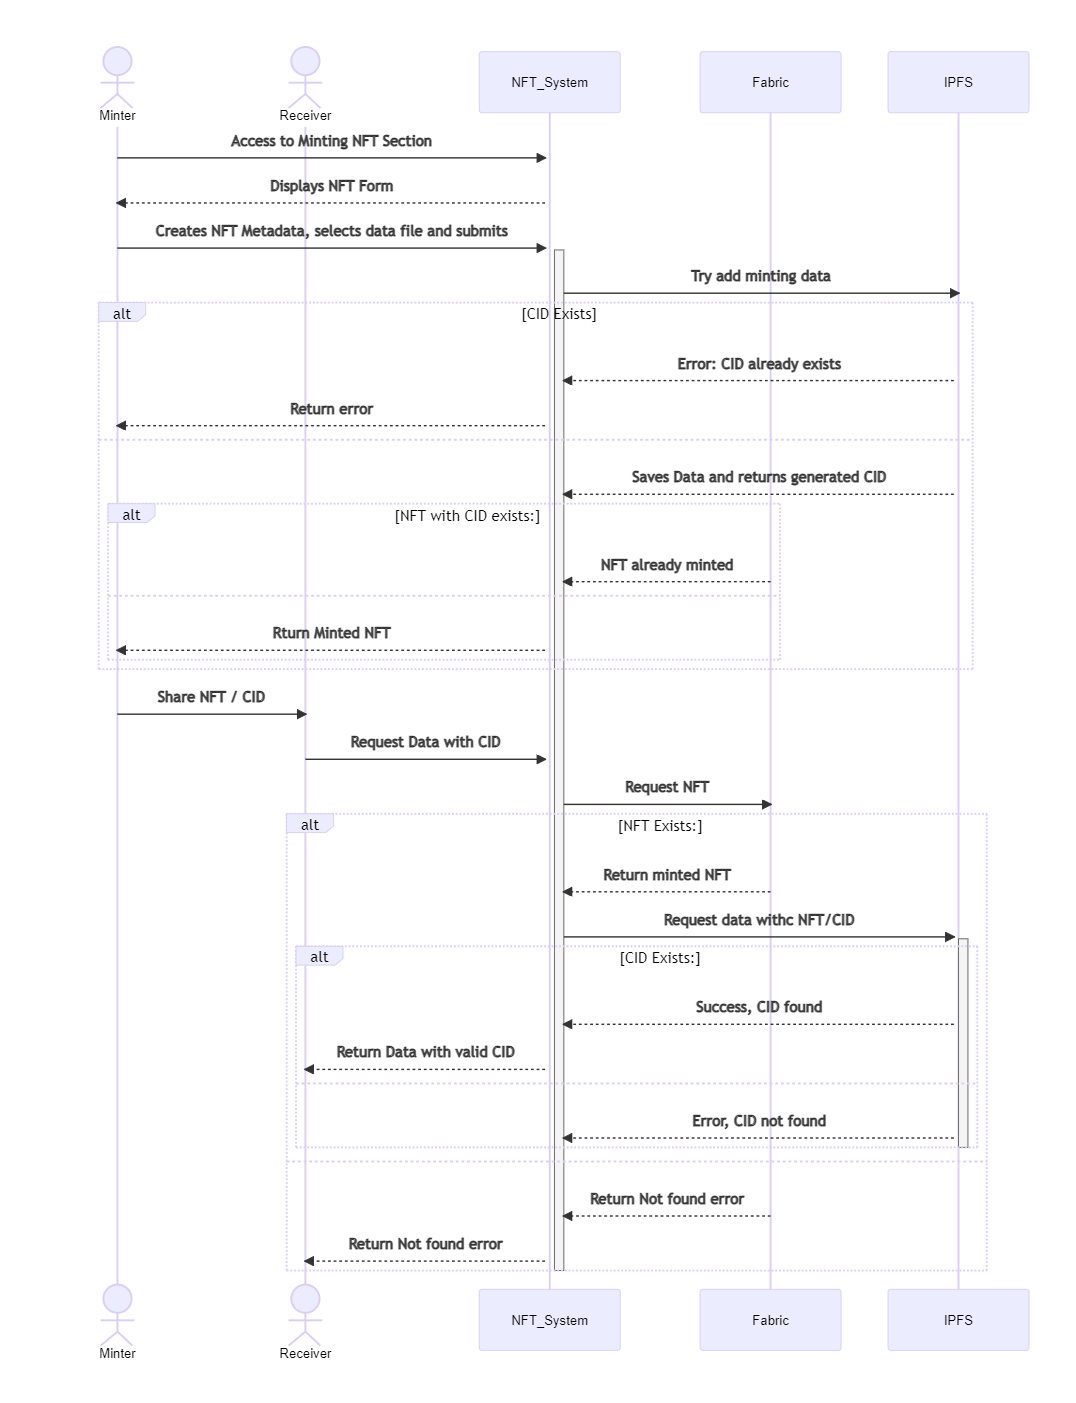
\includegraphics[width=15cm]{img/SequenceDiagram_MintNFT.png}
        \caption{Sequence diagram to mint a \ac{NFT}}
        \label{fig:SeqDiag_Mint}
    \end{figure}
    
 \begin{figure}[!h]
        \centering
        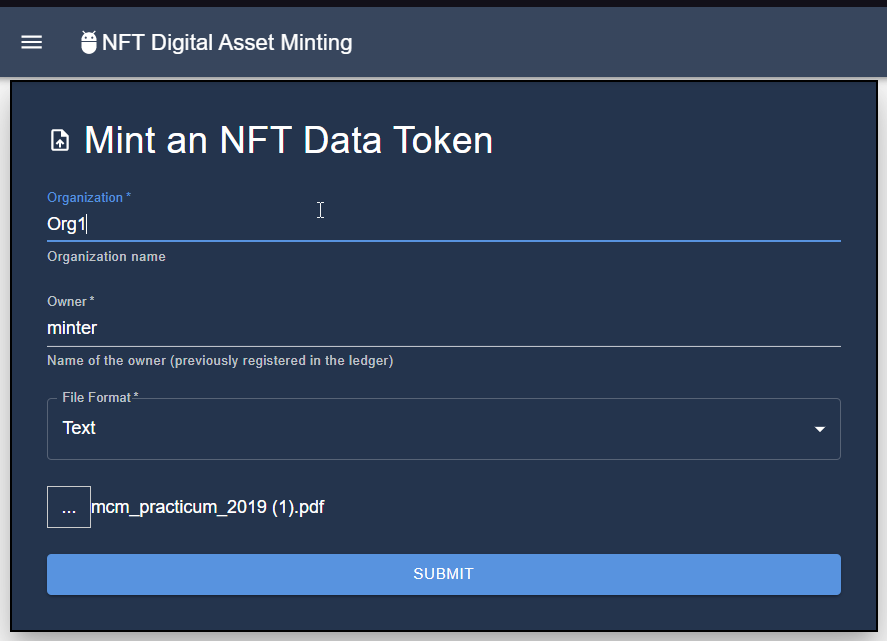
\includegraphics[width=10cm]{img/UIMinting.png}
        \caption{Front-end showing minting process.}
        \label{fig:UI_Mint}
    \end{figure}

 \begin{figure}[!h]
        \centering
        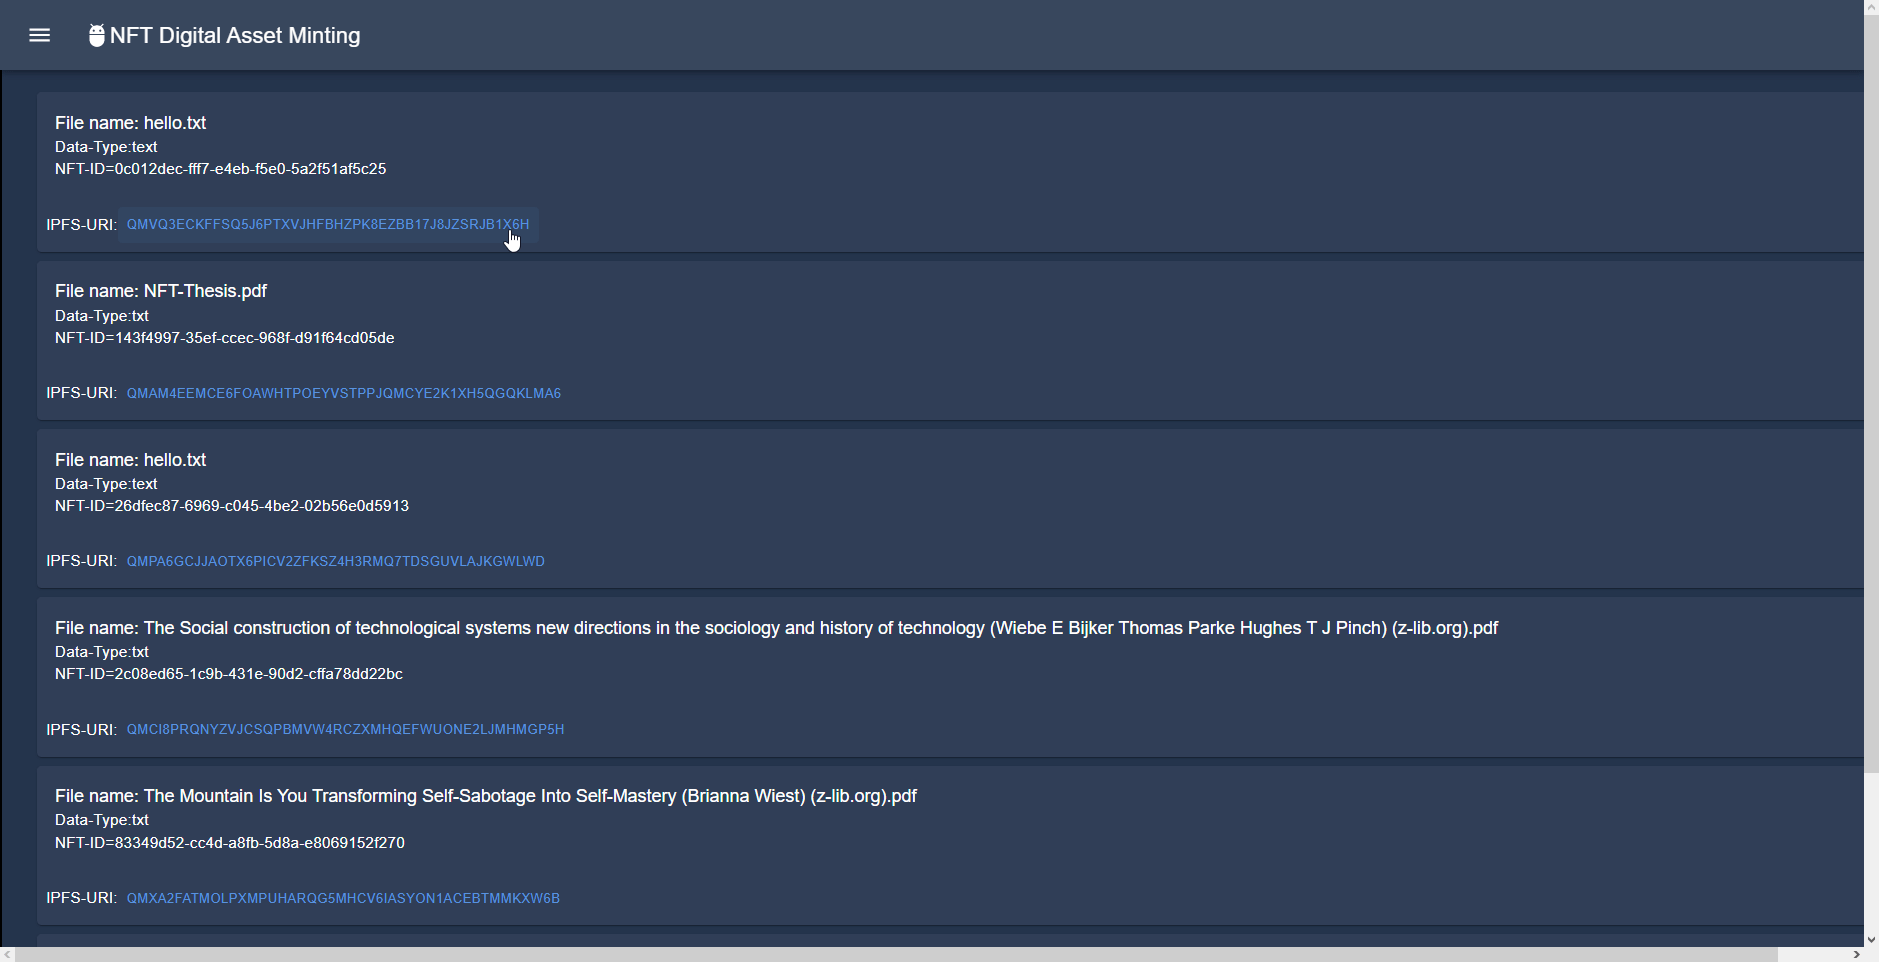
\includegraphics[width=15cm]{img/SystemList.png}
        \caption{Front-end showing minted \ac{NFT}s in the system.}
        \label{fig:UI_MintTokens}
    \end{figure}
    
\subsection{NFT Transfer}
It is possible through the \ac{REST} \ac{API} to transfer the generated tokens from one owner to the other. This process will acknowledge that the new user is the new owner of the \ac{NFT}. It is possible then to track the chain of ownership.

\subsection{NFT Burning}
The system also supports burning an \ac{NFT}, which basically blocks the token and flags it as unusable. if that happens, burned \ac{NFT} and \ac{CID} data cannot be accessed via the platform.

IT is possible, however to access the data via the \ac{IPFS} server.